\section{Messung}
\renewcommand{\ort}{topics/SPSchaltungen}


\subsection{Prototypfilter/Referenzfilter}

\fb \\
$Z_0 = 1 \Omega$
Normierung: bei $\omega_{ref} = \omega_c$:
\begin{pitemize}
    \item $\omega_c C = 2\Omega^{-1}$
    \item $\omega_c L = 1\Omega$
\end{pitemize}

\fb \\
$\abs{S_{21}(\omega_c)}^2 = \frac{1}{2}$


\subsection{Leitungsfilter}
für HF-Filter Übergang zu Leitungselementen

\fb\\

$Z_1 = Z_L \frac{Z_2 + jZ_L \tan(\beta l)}{Z_L + j Z_2\tan(\beta l)}$\\
$\beta l = \Theta = \frac{2\pi}{\lambda} l = \frac{2\pi}{\lambda} \frac{\lambda}{4} \frac{\omega}{\omega_0} = \frac{\pi}{2} \frac{\omega}{\omega_0}$

\fb Kurzschliessen von $Z_2$ \\

$Z_2 = 0 \Rightarrow Z_{1,KS} = jZ_L \tan(\beta l) \hat{=}$ induktiv
$Z_L \hat{=} \tilde{L}$ \\
\fb Leerlauf \\

$Z_2 \rightarrow \infty \Rightarrow Z_{1,LL} = Z_L \frac{1}{j\tan(\beta l)} \hat{=}$ kapazitiv
$Z_L \hat{=} \frac{1}{\tilde{C}}$ 

$\frac{w_c}{\omega_{ref} C} \Rightarrow \tilde{C} = C$\\

für $L = \tilde{L}$ und $C = \tilde{C}$:\\
\begin{equation}
\frac{\omega_{ref}}{\omega_c} = \tan(\beta l) = \tan(\frac{\pi}{2}\frac{\omega}{\omega_c})
\Leftrightarrow \omega = \omega_0 \frac{2}{\pi} \arctan(\frac{\omega_{ref}}{\omega_c})
\end{equation}

$\omega_{ref} \hat{=}$ Frequenz des Referenzfilter\\
$\omega$ ist die Frequenz des Leitungsfilters


\fb \\
\begin{pitemize}
\item $\omega_{ref} = 0 \Rightarrow \omega = 0$
\item $\omega_{ref} \rightarrow \infty \Rightarrow \omega = \omega_0 \frac{\pi}{2}\frac{2}{\pi} = \omega_0$
\item $\omega_{ref} = \omega_c \Rightarrow \omega = \omega_0 \frac{2}{\pi} \arctan(1) = \frac{\omega_0}{2}$
\end{pitemize}

2Draht-ESB:\\
\fb \\

Konzentrierte Elemente ersetzen durch Stichleitungen.
\begin{pitemize}
    \item Indiktivitäten: Am Ende KS Stichleitungen 
    \item \fb
    \item \fb
    \item Kapazitäten: Am Ende LL Stichleitungen
\end{pitemize}


\subsection{Butterworth-Hochpassfilter}
Prototypfilter:
\fb \fb\\


Übergang zum Leitungsfilter
\fb \fb\\

bei Mikrostreifenleitungen sind keine seriel liegenden Stichleitungen möglich.

\subsection{Kuroda Identitäten}

\fb \\

$S = j \tan{\beta L}$ Richardstransformation

$\frac{1}{\sqrt{1 - s^2}}\begin{bmatrix}
    1 & sL \\ 0 & 1
\end{bmatrix} \begin{bmatrix}
    1 & sZ_0 \\ \frac{s}{Z_0} & 1
\end{bmatrix} \overset{!}{=} \frac{1}{\sqrt{1 - s^2}}\begin{bmatrix}
    1 & sZ_1 \\ \frac{s}{Z_1} & 1
\end{bmatrix}\begin{bmatrix}
    1 & 0 \\ sC & 1
\end{bmatrix}$ \\

$\begin{bmatrix}
    q + s^2\frac{L}{Z_0} & s(L + Z_0) \\ \frac{s}{Z_0} & 1
\end{bmatrix} \overset{!}{=} \begin{bmatrix}
    1 + s^2Z_1C & sZ_1 \\ s(\frac{1}{Z_1} + C) & 1
\end{bmatrix} $

\begin{pitemize}
    \item $\frac{L}{Z_0} = Z_1 C$
    \item $Z_1 = L + Z_0$
    \item $\frac{1}{Z_0} = \frac{1}{Z_1} + C$
    \item $n = 1 + \frac{L}{Z_0}$
    \item $Z_1 = nZ_0$
    \item $C = \frac{n-1}{n} \frac{1}{Z_0}$
\end{pitemize}


\subsubsection{Leitungsfilter}
\fb\\
Realisierung in Mikrostreifenleitungen.
Problem: 
\begin{pitemize}
    \item serielle Elemente nicht realisirbar.
    \item Leitungsverzweigung ggf. problematisch
\end{pitemize}

Anwedung der Kuroda-Identitäten. \\
Einfügen von Leitungselementen mit $Z_0$ von außen. $\Rightarrow$ keine Veränderung des Betrages, nur Phaseveränderung.

\fb \\

\fb \fb\\




\subsection{LC- Tiefpass mit Butterworthverhalten}
\begin{tikzpicture}[scale=.2, transform shape]
  % Coordinates
  \coordinate (A) at (0.00, 0.00);
  \coordinate (B) at (18.00, 0.00);
  \coordinate (C) at (1.02, -1.03);
  \coordinate (D) at (1.02, 8.14);
  \coordinate (E) at (1.00, 6.00);
  \coordinate (F) at (17.00, 0.00);
  \coordinate (G) at (14.75, 6.25);
  \coordinate (H) at (3.00, 0.00);
  \coordinate (I) at (9.00, 6.00);
  \coordinate (J) at (9.00, 0.00);
  \coordinate (K) at (8.99, 0.05);
  \coordinate (L) at (9.01, 6.05);
  \coordinate (M) at (8.99, 0.04);
  \coordinate (N) at (17.04, -0.05);

  % Drawing
  \draw[-Stealth] (A) -- (B);
  \draw[-Stealth] (C) -- (D);
  \draw[thick] (E) .. controls (14.75, 6.25) and (3.00, 0.00) .. (F);
  \draw[lightgray, thick, dashed] (E) -- (I);
  \draw[lightgray, thick, dashed] (K) -- (L);
  \draw[lightgray, thick, dashed] (M) -- (N);
  \node[above] at (I) {Ideal};
  \node[left, font=\Huge] at (E) {$\left|S_{21}\right|^2$};
  \node[below, font=\Huge] at (B) {$\omega_{ref}$};
  \node[below, font=\Huge] at (J) {$\omega_c$};
\end{tikzpicture}

\begin{pitemize}
    \item $\abs{S_{21}}^2 \max_{\mathrm{bei } \omega = 0}\limits$ flach
    \item $\abs{S_{21}(\omega_c)}^2 = \frac{1}{2}$
\end{pitemize}

Annahme: Verlustlosigkeit $\Rightarrow \abs{S_{11}}^2 + \abs{S_{21}}^2 = 1$
\\$\Rightarrow \abs{S_{21}}^2 = \frac{\abs{S_{21}}^2}{\abs{S_{21}}^2 +\abs{S_{11}}^2} = \frac{1}{1 + \frac{\abs{S_{11}}^2}{\abs{S_{21}}^2}} = \frac{1}{1 + \abs{\Sigma_{21}}^2} = \frac{1}{1 + Q_m(y)}$

mit $y = \left(\frac{\omega_{ref}}{\omega_c}\right)^2$ und $Q_m = a_0 + a_1y + a_2y^2 + ... + a_my^m$

$(m-1)$: Ableitung von $\abs{S_{21}}^2$ bei $y = 0 \Rightarrow$ verschwinden

\begin{pitemize}
    \item $\left(\frac{1}{1 + Q_m(y)}\right)' |_{y=0} \overset{!}{=} 0$
    \item $\left(\frac{1}{1 + Q_m(y)}\right)'' |_{y=0} \overset{!}{=} 0 \Rightarrow a_2 = 0$
    \item $\Rightarrow a_m \ne 0$
\end{pitemize}

$Q_m(y) = a_0 + a_my^m$
\begin{penumerate}
    \item $\abs{S_{21}(0)}^2 \overset{!}{=} 1 \Rightarrow \frac{1}{1 + a_0} = 1 \Rightarrow a_0 = 0$
    \item $\abs{S_{21}(1)}^2 \overset{!}{=} \frac{1}{2} \Rightarrow \frac{1}{1 + a_m} = \frac{1}{2} \Rightarrow a_m = 1$ bei $\omega_{ref} = \omega_c$
\end{penumerate}

$\abs{S_{21}}^2 = \frac{1}{1 + y^m}$

mit $y = \left(\frac{\omega_{ref}}{\omega_c}\right)^2 \Rightarrow$ Leitungsfilter $S \hat{=} j\omega_{ref}$, $S_c \hat{=} j\omega_{c}$

$\abs{S_{21}}^2 = \frac{1}{1 + \left(\frac{S}{S_c}\right)^{2m}}$

geg.: bschreibende Funktion (hier $\abs{S_{21}}^2$) $\Rightarrow$ Ziel: Realisierung mit L und c

\begin{tikzpicture}[scale=1, transform shape]
  % Coordinates
  \coordinate (A) at (-0.02, 1.04);
  \coordinate (B) at (0.00, 2.00);
  \coordinate (C) at (0.00, 0.00);
  \coordinate (M) at (4.25, 0.00);
  \coordinate (N) at (4.25, 2.00);
  \coordinate (O) at (4.25, 0.50);
  \coordinate (P) at (4.25, 1.50);
  \coordinate (Q) at (4.92, 0.45);
  \coordinate (D) at (1.50, 2.00);
  \coordinate (E) at (1.50, 0.00);
  \coordinate (F) at (3.50, 0.00);
  \coordinate (G) at (3.50, 2.00);
  \coordinate (H) at (2.51, 1);

  % Drawing
  \node[left, font=\Large] at (A) {$W_{in} \Rightarrow$};
  \draw (B) circle (0.10);
  \draw (C) circle (0.10);
  \draw (4,0.5) rectangle (4.5,1.5);
  \draw (M) -- (O);
  \draw (N) -- (P);
  \node[above] at (Q) {$Z_0$};
  \draw (1.5,-0.5) rectangle (3.5,2.5);
  \draw (B) -- (D);
  \draw (C) -- (E);
  \draw (F) -- (M);
  \draw (N) -- (G);
  \node[above, font=\Huge] at (H) {$?$};
\end{tikzpicture}

$W_{in}(s) = \frac{1 - S_{11}(s)}{1 + S_{11}(s)}$

$\abs{S_{11}}^2 = 1 - \abs{S_{21}}^2 = 1 - \frac{1}{1 + \left(\frac{S}{S_c}\right)^{2m}} = \frac{\left(\frac{S}{S_c}\right)^{2m}}{1 + \left(\frac{S}{S_c}\right)^{2m}}$

$\abs{S_{11}}^2 = S_{11}(s) S_{11}(-s)$

$S_{11}(s)$ Pole in linker s-HE für Stabilität


\subsubsection{Beispiel}
$s_c = j$, $m = 3$

$\abs{S_{11}}^2 = \frac{\left(-jS\right)^6}{1 + \left(-jS\right)^6} = \frac{-s^6}{1 - s^6} = S_{11}(s) S_{11}(-s) 
= \frac{\mp s^3}{-s^3 + 2s^2 - 2s + 1} \frac{\pm s^3}{s^3 + 2s^2 + 2s + 1}$ $S_{11}(s)$ ist zweiter frac


$W_{in}(s) = \frac{1 - S_{11}(s)}{1 + S_{11}(s)}$

Wahl des negative VZ $\Rightarrow W_{in}(s) = \frac{s^3 + 2s^2 + 2s + 1 - s^3}{s^3 + 2s^2 + 2s + 1 + s^3}$
\begin{pitemize}
    \item $\lim_{s\rightarrow\infty}\limits W_{in}(s) = \frac{1}{s} \Rightarrow C = 1$
\end{pitemize}

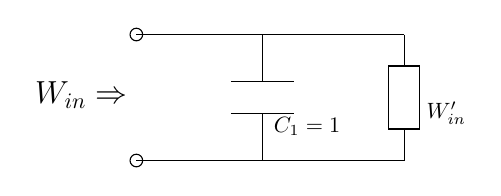
\begin{tikzpicture}[scale=0.8, transform shape]
  % Coordinates
  \coordinate (A) at (-0.02, 1.04);
  \coordinate (L) at (2.71, 0.27);
  \coordinate (B) at (0.00, 2.00);
  \coordinate (C) at (0.00, 0.00);
  \coordinate (D) at (2.00, 0.00);
  \coordinate (E) at (2.00, 2.00);
  \coordinate (F) at (1.50, 1.25);
  \coordinate (G) at (2.50, 1.25);
  \coordinate (H) at (1.50, 0.75);
  \coordinate (I) at (2.50, 0.75);
  \coordinate (J) at (2.00, 0.75);
  \coordinate (K) at (2.00, 1.25);
  \coordinate (M) at (4.25, 0.00);
  \coordinate (N) at (4.25, 2.00);
  \coordinate (O) at (4.25, 0.50);
  \coordinate (P) at (4.25, 1.50);
  \coordinate (Q) at (4.92, 0.45);

  % Drawing
  \node[left, font=\Large] at (A) {$W_{in} \Rightarrow$};
  \node[above] at (L) {$C_1=1$};
  \draw (B) circle (0.10);
  \draw (C) circle (0.10);
  \draw (C) -- (D);
  \draw (B) -- (E);
  \draw (F) -- (G);
  \draw (H) -- (I);
  \draw (D) -- (J);
  \draw (E) -- (K);
  \draw (D) -- (M);
  \draw (E) -- (N);
  \draw (4,0.5) rectangle (4.5,1.5);
  \draw (M) -- (O);
  \draw (N) -- (P);
  \node[above] at (Q) {$W_{in}'$};
\end{tikzpicture}  

$W_{in}(0) = 1 \hat{=}$ Durchlassbereich


$W_{in} = \frac{1}{V_{in}}$\\
Wechsel in Admittanzebene: $V_{in} = sC_1 + V_{in}' \Leftrightarrow V_{in}' = V_{in} -s = \frac{2 s^3 + 2s^2 + 2s + 1 - 2s^3 - 2s^2 - s}{2s^2 + 2s + 1} = \frac{s + 1}{2s^2  + 2s + 1}$

$W_{in}' = \frac{2s^2 + 2s + 1}{s + 1}$

$\lim_{s \rightarrow \infty} W_{in}(s)' = 2s \Rightarrow$  induktiv $L = 2$

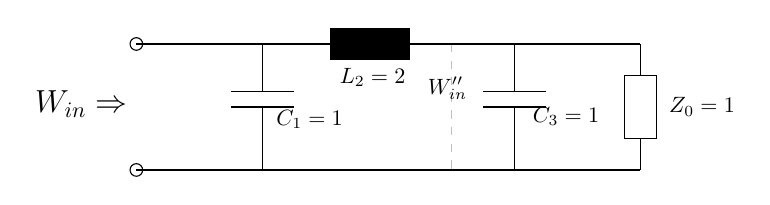
\begin{tikzpicture}[scale=0.8, transform shape]
  % Coordinates
  \coordinate (A) at (-0.02, 1.04);
  \coordinate (L) at (2.75, 0.53);
  \coordinate (B) at (0.00, 2.00);
  \coordinate (C) at (0.00, 0.00);
  \coordinate (D) at (2.00, 0.00);
  \coordinate (E) at (2.00, 2.00);
  \coordinate (F) at (1.50, 1.25);
  \coordinate (G) at (2.50, 1.25);
  \coordinate (H) at (1.50, 1.00);
  \coordinate (I) at (2.50, 1.00);
  \coordinate (J) at (2.00, 1.00);
  \coordinate (K) at (2.00, 1.25);
  \coordinate (M) at (5.00, 0.00);
  \coordinate (N) at (5.00, 2.00);
  \coordinate (O) at (3.75, 1.20);
  \coordinate (P) at (4.94, 0.99);
  \coordinate (Q) at (6.82, 0.58);
  \coordinate (R) at (5.50, 1.25);
  \coordinate (S) at (6.50, 1.25);
  \coordinate (T) at (5.50, 1.00);
  \coordinate (U) at (6.50, 1.00);
  \coordinate (V) at (6.00, 1.00);
  \coordinate (W) at (6.00, 1.25);
  \coordinate (X) at (6.00, 0.00);
  \coordinate (Y) at (6.00, 2.00);
  \coordinate (Z) at (8.00, 0.00);
  \coordinate (AA) at (8.00, 2.00);
  \coordinate (AB) at (8.00, 0.50);
  \coordinate (AC) at (8.00, 1.50);
  \coordinate (AD) at (8.98, 0.73);

  % Drawing
  \node[left, font=\Large] at (A) {$W_{in} \Rightarrow$};
  \node[above] at (L) {$C_1=1$};
  \draw (B) circle (0.10);
  \draw (C) circle (0.10);
  \draw (C) -- (D);
  \draw (B) -- (E);
  \draw (F) -- (G);
  \draw (H) -- (I);
  \draw (D) -- (J);
  \draw (E) -- (K);
  \draw (D) -- (M);
  \draw (E) -- (N);
  \draw[fill=black] (3.09,1.75) rectangle (4.34,2.25);
  \node[above] at (O) {$L_2 = 2$};
  \draw[lightgray, dashed] (N) -- (M);
  \node[above] at (P) {$W_{in}''$};
  \node[above] at (Q) {$C_3
=1$};
  \draw (R) -- (S);
  \draw (T) -- (U);
  \draw (X) -- (V);
  \draw (Y) -- (W);
  \draw (M) -- (Z);
  \draw (N) -- (AA);
  \draw (7.75,0.5) rectangle (8.25,1.5);
  \draw (Z) -- (AB);
  \draw (AA) -- (AC);
  \node[above] at (AD) {$Z_0 = 1$};
\end{tikzpicture}

$W_{in}' = sL_2 + W_{in}'' \Rightarrow W_{in}'' = W_{in}' - sL_2 = \frac{2s^2 + 2 + 1 - 2s^2 - 2s}{s + 1} = \frac{1}{s + 1}$

$V_{in}'' = \frac{1}{W_{in}''} = s + 1 \hat{=} $ Parallelschaltung $C_3 = 1$ und $Z_0 = 1$


Wahl des positiven VZ: 
$W_{in} = \frac{s^3 + 2s^2 + 2s + 1 + s^3}{s^3 + 2s^2 + 2s + 1 - s^3} = \frac{2s^3 + 2s^2 + 2s + 1}{2s^2 + 2s + 1}$
Noch immer TF, da $W_{in}(0) = 0$


\begin{pitemize}
    \item $\lim_{s\rightarrow\infty} W_{in} = s \Rightarrow$ induktiv $L_1 = 1$
    \item $W_{in} = sL_1 + W_{in}' \Rightarrow W_{in}' = \frac{2s^3 + 2s^2 + 2s + 1 - 2s^3 - 2s^2 - s}{2s^2 + 2s + 1} = \frac{s + 1}{2s^2 + 2s + 1}$
    \item $\lim_{s\rightarrow\infty} W_{in}' = \frac{1}{2s} \Rightarrow$ kapazitiv $C_2 = 2$
    \item $V_{in}' = sC_2 + V_{in}'' \Rightarrow V_{in}'' = \frac{2s^2 + 2s + 1 - 2s^2 - 2s}{s + 1}$
\end{pitemize}



\subsection{LC-Hochpassfilter mit Butterworthverhalten}

vom TP: $\abs{S_{21}}^2 = \frac{1}{1 + \left(\frac{s}{s_C}^{2m}\right)}$
Übergang zum HP durch subsitution $s->\frac{1}{s}$
HP: $\abs{S_{21}}^2 = \frac{1}{1 + \left(\frac{s_C}{s}^{2m}\right)}$

\subsubsection{Beispiel}

$m = 3$, $s_c = j $

$\abs{S_{21}}^2 = \frac{1}{1 + \frac{-1}{s^6}} = \frac{s^6}{s^6 - 1}$

$\abs{S_{11}}^2 = 1 - \abs{S_{21}}^2 = \frac{-1}{s^6 -1} = \frac{1}{1 - s^6} = S_{11}(s) S_{11}(-s)$
$S_{11}(s) = \frac{\pm 1}{s^3 + 2s^2 + 2s + 1}$

Wahl des pos. VZ $W_{in} = \frac{1 + S_{11}}{1 - S_{11}} = \frac{s^3 + 2s^2 + 2s + 1 + 1}{s^3 + 2s^2 + 2s + 1 - 1} = \frac{s^3 + 2s^2 + 2s + 2}{s^3 + 2s^2 + 2s}$

HP da $\lim_{s\rightarrow\infty} = 1$

\begin{pitemize}
    \item $\lim_{s\rightarrow0}\limits = \frac{2}{2s} = \frac{1}{s} \Rightarrow C = 1$
    \item Kapazität is serielle
    \item $W_{in}' = W_{in} - \frac{1}{s} = \frac{s^3 + 2s^2 + 2s + 2 - s^2 - 2s - 2}{s^3 + 2s^2 + 2s} = \frac{s^3 + s^2}{s^3 + 2s^2 + 2s} = \frac{s^2 + s}{s^2 + 2s + 2}$
    \item $\lim_{s\rightarrow0}\limits W_{in}' = \frac{s}{2} \Rightarrow L = \frac{1}{2}$
    \item Indiktivität ist parallel 
    \item $V_{in}'' = V_{in}' - sL = \frac{s^2 + 2s + 2 - 2s - 2}{s^2 + s} = \frac{1}{1 + s} \Rightarrow$ Reihenschaltung aus $C = 1$ und $Z_0 = 1$ 
\end{pitemize}






\subsection{Filter aus Induktivitäten und Kapazitäten sowie Leitungselementen}
\bildf{z_img_4}

nicht rendudant

\bildf{z_img_5}

rendudant

beschreibenede Funktion für Butterworth

$\left[K_{UE}\right] = \frac{1}{\sqrt{1 - s^2}}\begin{bmatrix}
    1 & sZ_2 \\ \frac{s}{Z_2} & 1
\end{bmatrix}$

$\begin{bmatrix}
    A & B \\ C & D
\end{bmatrix} = \begin{bmatrix}
    1 & sL_1 \\ 0 & 1
\end{bmatrix} \frac{1}{\sqrt{1 - s^2}} \begin{bmatrix}
    1 & sZ_2 \\ \frac{s}{Z_2} & 1
\end{bmatrix}\begin{bmatrix}
    1 & sL_3 \\ 0 & 1
\end{bmatrix}\begin{bmatrix}
    1 & 0 \\ sC_4 & 1
\end{bmatrix}$

$\left(\frac{1}{\sqrt{1 -s^2}}\right)^n P_{m+n}(s)$

n: Anzahl Leitungselementen
m: Anzahl and Indiktivitäten and Kapazitäten



$\abs{S_{21}(s)}^2 = \frac{1}{1 + \abs{\Sigma_{21}(s)}^2}$

$\abs{\Sigma_{21}(s)}^2 = \left(\frac{s^2}{s_c^2}\right)^m \left(\frac{s^2}{s_c^2}\right)^n \frac{\left(1 - s_c^2\right)^n}{\left(1 - s^2\right)^n}$ TP mit Butterworth


geg:: $W_{in}(s)$:

\bildf{z_img_3}
$W_{in} = Z_1 \frac{W_1(s) + sZ_1}{Z_1 + sW_1(s)}$

Auflösen nach $W_1(s)$: 
$W_1(s) = \frac{Z_1 (sZ_1 - W_{in})}{sW_{in} - Z_1}$

$W_{in}(s=1) = Z_1 \frac{W_1(1) + Z_1}{Z_1 + W_1(1)} = Z_1$


Zum Zeitpunkt t=0s => Spannungssprung am Leitungsanfang $\rightarrow t = 0 \rightarrow$ Verhältnis von Spannung zu Strom $\hat{=}$ Leitungswellenwiderstand $Z_1$

Grenzwertsatz der Laplace-Transformation: $f(0+) = \lim_{p\rightarrow\infty} \limits p F(p)$ mit $p = j\omega \Leftrightarrow \omega = -jp$

mit $s = j \tan(\frac{\pi}{2} \frac{\omega}{\omega_0}) = j \tan(\frac{\pi}{2} \left(\frac{-jp}{\omega_0}\right))$

$\lim_{p\rightarrow\infty} \limits j \tan(\frac{\pi}{2} \left(\frac{-jp}{\omega_0}\right)) = 1 \Rightarrow p \rightarrow \infty \hat{=} s \rightarrow 1$

$W_{in}(s) = W_{in}(1) \frac{sW_{in}(1) - W_{in}(s)}{sW_{in}(s) - W_{in}(1)}$

Zähler und Nenner NS bei s = 1 und s= -1s

$(1+s)(1-s) = (1-s^2)$


\subsubsection{Beispiel}

$W_{in}(s) = \frac{1 + 3s + \frac{1}{2}s^2}{1 + \frac{3}{2}s + 2 s^2}$

\begin{penumerate}
    \item Ist ein UE enthalten? $W_{in}(1) \overset{!}{=} - W_{in}(-1)$
    \begin{pitemize}
        \item $W_{in}(1) = \frac{1 + 3 + \frac{1}{2}}{1 + \frac{3}{2} + 2} = 1 = Z_1$
        \item $-W_{in}(1) = -\frac{1 - 3 + \frac{1}{2}}{1 - \frac{3}{2} + 2} = 1$
        \item \bildf{z_img_6}
    \end{pitemize}
    \item Abspaltung
    \begin{pitemize}
        \item $W_{in}'(s) = \frac{s - \frac{1 + 3s + \frac{1}{2}s^2}{1 + \frac{3}{2}s + 2 s^2}}{\frac{1 + 3s + \frac{1}{2}s^2}{1 + \frac{3}{2}s + 2 s^2} - 1} = \frac{s + \frac{3}{2}s^2 + 2s^3 - 1 - 3s - \frac{1}{2}s^2}{s + 3s^2 + \frac{1}{2}s^3 -1-3s -2s^2} = \frac{2s^3 + s^2 - 2s - 1}{\frac{1}{2}s^3 + s^2 - \frac{1}{2}s - 1} = \frac{2s + 1}{\frac{1}{2}s + 1}$
    \end{pitemize}
    \item Ist UE enthalten
    \begin{pitemize}
        \item $W_{in}'(1) = \frac{3}{\frac{3}{2}} = 2 = Z_2$
        \item $-W_{in}+(-1) = -\frac{-1}{\frac{1}{2}} = 2$
        \item \bildf{z_img_7}
    \end{pitemize}
    \item Abspaltung
    \begin{pitemize}
        \item $W_{in}''(s) = 2\frac{s2 - \frac{2s + 1}{\frac{1}{2}s + 1}}{s\frac{2s + 1}{\frac{1}{2}s + 1} - 2} = 2\frac{s^2 + 2s - 2s - 1}{2s^2 + s - s - 2} = \frac{s^2 - 1}{s^2 - 1} = 1$
    \end{pitemize}
\end{penumerate}




\subsection{Beispiel}

$W_{in}(s) = \frac{1 + 3s + \frac{1}{2}s^2}{1 + \frac{1}{2}s}$

\begin{penumerate}
    \item $W_{in}(1) = -W_{in}(-1)$:
    \begin{pitemize}
        \item $W_{in}(1) = \frac{1 + 3 + \frac{1}{2}}{1 + \frac{1}{2}} = 3 = Z_1$
        \item $W_{in}(-1) = \frac{1 - 3 + \frac{1}{2}}{1 - \frac{1}{2}} = -3$
        \item \bildf{z_img_1}
    \end{pitemize}
    \item Abspaltung: $W_{in}'(s) = \frac{3 (3s - \frac{1 + 3s + \frac{1}{2}s^2}{1 + \frac{1}{2}s})}{s\frac{1 + 3s + \frac{1}{2}s^2}{1 + \frac{1}{2}s} - 3} = 3\frac{3s + \frac{3}{2}s^2 - 1 - 3s - \frac{1}{2}s^2}{s + 3 s^2 + \frac{1}{2}s^3 - 3 - \frac{3}{2}s} = 3\frac{s^2 - 1}{\frac{1}{2}s^3 + 3s^2 - \frac{1}{2}s - 3} = \frac{3}{2}\frac{s^2 - 1}{s^3 + 6s^2 - s - 6} = \frac{3}{2} \frac{s^2 -1}{(s^2 - 1)(s + 6)} = \frac{3}{2} \frac{1}{s + 6}$
    \item $V_1(s)' = \frac{1}{6}s + 1$ : Parallelschaltung aus $C$ und $Z_0$ 
\end{penumerate}


\subsubsection{Beispiel}

\bildf{z_img_2}

$W_{in} = s \frac{\frac{1}{s} s}{\frac{1}{s} + s}$

Überprüfung mit Realisierung